\documentclass{report}   %Documento tipo reporte
\usepackage[spanish]{babel}    %Paquete de Idioma
\usepackage{float, graphicx, caption, color, amsmath}
\usepackage[hidelinks]{hyperref}

\begin{document}


\begin{titlepage}    %Portada
	\centering
	{\huge\bfseries Proyecto de investigación: \par}
	\vspace{1cm}
	{\huge\bfseries  Interrupciones \par}
    \vspace{3cm}
    {\scshape\large Valentina Botero Vivas \par}
    \vspace{3cm}
      {\scshape\large Docente  \par}
	\vspace{0.5cm}
    {\scshape\large Augusto Salazar Jimenez  \par}
	\vspace{3cm}
	 {\scshape\large Universidad de Antioquia \par}
	\vspace{1cm}
    {\scshape\large Informática II  \par}
	\vspace{1cm}
	{\large 3 de Julio del 2020 \par}
\end{titlepage}


Una interrupción o petición de interrupción es una señal recibida por el procesador que le indica suspender la ejecución actual y ejecutar una tarea específica para tratarla.\\

Entonces, la interrupción viene determinada por la ocurrencia de la señal, la cual provoca un desvío a una dirección específica de memoria, esto interrumpe momentánamente la ejecución del programa . A partir de esta dirección se enccuentra la rutina de tratamiento que se encarga de realizar la operación,devolviendo después el control al punto interrumpido del programa. Este proceso se ilustra en la figura \ref{fig:Interrupción}

\begin{figure}[H]
      \centering
      \captionsetup{justification=centering}
      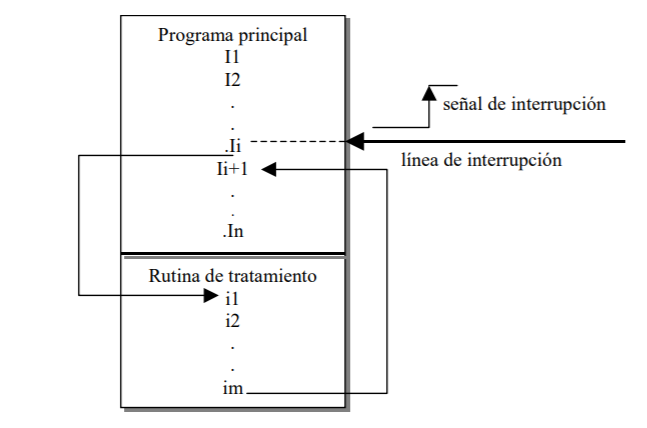
\includegraphics[width=0.8\textwidth]{1.PNG}
      \caption{Interrupción ocasionada por señal externa. Tomado de \cite{3}}
      \label{fig:Interrupción}
   \end{figure}

Las interrupciones son de gran importancia ya que aumentan el rendimiento de los sistemas. 

\section*{Historia}
Si se busca hablar de la historia de las interrupciones, es importante aclarar que éstas fueron necesarias y aparecieron como solución a un problema.\\\\
Surgen de las necesidades que tienen los dispositivos periféricos de enviar información al procesador principal de un sistema de computación.\\\\ Por ejemplo, en los primeros sistemas cuando una aplicación necesitaba leer la pulsación de una tecla, interrogaba continuamente al teclado es decir, sondeaba el dispositivo cada cierto tiempo hasta que la tecla fuera presionada, teniendo en cuenta que mientras se esperaba una tecla, no se podían ejecutar otras tareas.\\ La solución a este problema apareció con la llamada interrupción de teclado en donde el controlador del dispositivo, en este caso el teclado, es quien genera una interrupción sólo cuando el dispositivo está listo para transferir datos.\\ En este caso, el microprocesador, no sondeaa ningún dispositivo, sino que queda a la espera de que estos le avisen (le "interrumpan") cuando deba ejecutar una subtarea.

\section*{Tipos de interrupciones}
Las interrupciones pueden ser:
\item Síncrónicas: 
Debido a la fuente que los produce, pueden clasificarse en tres tipos:
\begin{enumerate}
 \item Excepciones:


\item Excepciones.
\item Interrupciones de hardware.
\item Interrupciones de software.
\end{enumerate}


\begin{thebibliography}{0}
  \bibitem {1}Concepto de interrupciones. (s.f) .Lenguaje ensamblador.
  https://leo-yac.wixsite.com/lenguaje-ensamblador/el-concepto-de-interrupciones
  \bibitem{2} Jorge Luis Tinoco.(2011). Interrupciones del microprocesador. https://es.slideshare.net/jorg-leoxd/interrupciones-del-microprocesador
  \bibitem{3} Interrupciones.(s.f). Estructura de computadores,Facultad de Informática,UCM. http://www.fdi.ucm.es/profesor/jjruz/WEB2/Temas/Curso05-06/EC9.pdf
\end{thebibliography}

\end{document}
